\documentclass{article}
\usepackage[T1]{fontenc}
\usepackage[french]{babel}
\usepackage{amssymb}
\usepackage{fullpage}
\usepackage{graphicx}
\usepackage{color}
%
% Environnement "exercice"
%
\newcounter{numexercice}
\newenvironment{exercice}{\addtocounter{numexercice}{1}\par\bigskip\noindent{\large \bf Exercice \thenumexercice\par}}{}
%
% Ensembles de nombres
%
\newcommand{\N}{\mbox{\rm I$\!$N}}
\newcommand{\Z}{\mbox{\rm \lower0.3pt\hbox{$\angle\!\!\!$}Z}}
\newcommand{\Q}{\mbox{\rm $~\vrule height6.5pt width0.5pt depth0.3pt\!\!$Q}}
\newcommand{\R}{\mbox{\rm I$\!$R}}
\newcommand{\C}{\mbox{\rm $~\vrule height6.5pt width0.5pt depth0.3pt\!\!$C}}
% 
%%%%%%%%%%%%%%%%%%%%%%%%%%%%%%%%%%%%%%%%%%%%%%%%%%%%%%%%%%%%%%%%%%
%
\title{\textbf{TD ASDO 2 : algorithme de Roy-Warshall (correction)}}
\begin{document}
\maketitle

\textbf{1. } 

\begin{equation}
  M \dotplus I = \left(
    \begin{array}{cccccc}
      1 & 1 && 1 & 1 & \\
      & 1 & 1 &&& \\
      & 1 & 1 & 1 && \\
      &&& 1 & 1 & \\
      &&& 1 & 1 & 1 \\
      &&& 1 & & 1 \\
    \end{array}
    \right)
\end{equation}

Aucun arc n'ayant pour extrémité $A$, $\theta_A$ ne peut ajouter aucun
arc au graphe $G$.

\begin{equation}
  M_1 = \theta_A(M \dotplus I) = \left(
    \begin{array}{cccccc}
      1 & 1 && 1 & 1 & \\
      & 1 & 1 &&& \\
      & 1 & 1 & 1 && \\
      &&& 1 & 1 & \\
      &&& 1 & 1 & 1 \\
      &&& 1 & & 1 \\
    \end{array}
    \right)
\end{equation}

Il existe un chemin de longueur 2, reliant $A$ à $C$ par $B$, on ajoute donc
l'arc $(A,C)$ au graphe. Il existe aussi un chemin de longueur 2
reliant $C$ à lui-même via $B$ mais ceci ne provoque aucun ajout dans
le graphe. 

\begin{equation}
  M_2 = \theta_B(M_1) = \left(
    \begin{array}{cccccc}
      1 & 1 & {\color{red} 1} & 1 & 1 & \\
      & 1 & 1 &&& \\
      & 1 & 1 & 1 && \\
      &&& 1 & 1 & \\
      &&& 1 & 1 & 1 \\
      &&& 1 & & 1 \\
    \end{array}
    \right)
\end{equation}

Les itérations suivantes sont décrites ci-après.

\begin{equation}
  M_3 = \theta_C(M_2) = \left(
    \begin{array}{cccccc}
      1 & 1 & 1 & 1 & 1 & \\
      & 1 & 1 & {\color{red} 1}&& \\
      & 1 & 1 & 1 && \\
      &&& 1 & 1 & \\
      &&& 1 & 1 & 1 \\
      &&& 1 & & 1 \\
    \end{array}
    \right)
\end{equation}

\begin{equation}
  M_4 = \theta_D(M_3) = \left(
    \begin{array}{cccccc}
      1 & 1 & 1 & 1 & 1 & \\
      & 1 & 1 & {1}& {\color{red} 1}& \\
      & 1 & 1 & 1 & {\color{red} 1} & \\
      &&& 1 & 1 & \\
      &&& 1 & 1 & 1 \\
      &&& 1 & {\color{red} 1} & 1 \\
    \end{array}
    \right)
\end{equation}

\begin{equation}
  M_5 = \theta_E(M_4) = \left(
    \begin{array}{cccccc}
      1 & 1 & 1 & 1 & 1 & {\color{red} 1}\\
      & 1 & 1 & {1}& { 1}& {\color{red} 1}\\
      & 1 & 1 & 1 & { 1} & {\color{red} 1}\\
      &&& 1 & 1 & {\color{red} 1}\\
      &&& 1 & 1 & 1 \\
      &&& 1 & { 1} & 1 \\
    \end{array}
    \right)
\end{equation}

\begin{equation}
  M_6 = \theta_F(M_5) = \left(
    \begin{array}{cccccc}
      1 & 1 & 1 & 1 & 1 & { 1}\\
      & 1 & 1 & {1}& { 1}& { 1}\\
      & 1 & 1 & 1 & { 1} & { 1}\\
      &&& 1 & 1 & { 1}\\
      &&& 1 & 1 & 1 \\
      &&& 1 & { 1} & 1 \\
    \end{array}
    \right)
\end{equation}

Les composantes fortement connexes de $G$ sont au nombre de trois :
$\{A\}$, $\{B,C\}$ et $\{D,E,F\}$, comme le montre la
figure~\ref{fig:cc}.

\begin{figure}[htbp]
  \begin{center}
    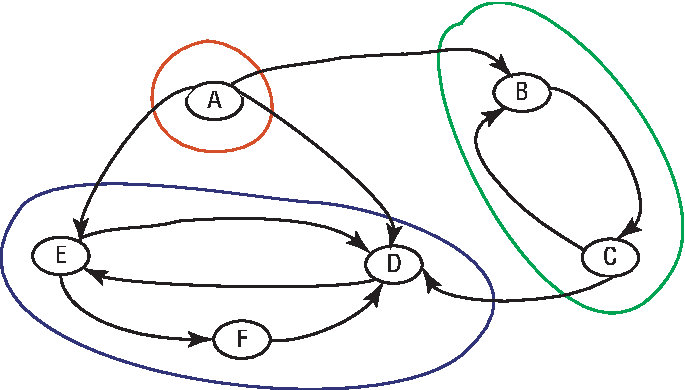
\includegraphics[width=6cm]{td_rw_cc.pdf}
    \caption{Graphe $G$}
    \label{fig:cc}
  \end{center}
\end{figure}

\textbf{2.1} Dans $\theta_r(G)$ figurera l'arc $(i,j)$ s'il existait
dans $G$ (i.e. $m_{ij} = 1$) ou bien si les arcs $(i,r)$ et $(r,j)$
appartiennent à $G$, c'est-à-dire si $m_{ir} = 1$ et $m_{rj} = 1$. En
utilisant l'addition et la multiplication booléenne, on obtient
immédiatement
\begin{equation}
  m_{ij}^{(r)} = m_{ij} \dotplus m_{ir}m_{rj}
\end{equation}

\textbf{2.2} Pour tout couple $(i,j)$, en utilisant la propriété
démontrée à la question précédente, on a

\begin{equation}
  \begin{array}{rcl}
  m_{ij}^{s\circ r} & = & m_{ij}^r \dotplus m_{is}^r m_{sj}^r \\
  & = & m_{ij} \dotplus m_{ir} m_{rj} \dotplus m_{is} m_{sj} \dotplus
  m_{is} m_{sr} m_{rj} \dotplus m_{ir} m_{rs} m_{sj} \\
  \label{eq:sym}
\end{array}
\end{equation}

L'équation (\ref{eq:sym}) étant symétrique en $s$ et $r$, la
commutativité est immédiate.

\textbf{2.3} En faisant $r=s$ dans l'équation (\ref{eq:sym}), on obtient
\begin{equation}
  \begin{array}{rcl}
  m_{ij}^{r\circ r} & = & 
  m_{ij} \dotplus m_{ir} m_{rj} \dotplus m_{ir} m_{rj} \dotplus
  m_{ir} m_{rr} m_{rj} \dotplus m_{ir} m_{rr} m_{rj} \\
  & = & m_{ij} \dotplus m_{ir}m_{rj} \\
  & = & m_{ij}^r \\
\end{array}
\end{equation}

d'où l'idempotence (d'ailleurs évidente par définition même de
$\theta_r$).

\textbf{2.4} Le calcul de $m_{ij}^{t(s\circ r)}$ donne une formule
symétrique en $r$, $s$ et $t$ : l'associativité de la composition des
opérateurs en découle.

\textbf{2.5} L'effet de $\theta$ est évident : pour chaque sommet $i$,
il ajoute les chemins de longueur 2 entre deux sommets passant par
$i$. Dès lors, $\theta^2$ a pour effet d'ajouter au graphe les chemins
de longueur inférieure ou égale à 3, et ainsi de suite...

$\theta^{n-2}$ a donc pour effet d'ajouter à $G$ les arcs $(i,j)$ qui
n'existent pas s'il existe dans $G$ un chemin de $i$ à $j$ de longueur
inférieure ou égale à $n-1$. La longueur maximale d'un chemin
élémentaire dans un graphe à $n$ sommets, on en déduit que
$\theta^{n-2}=\tau (G)$.

\textbf{2.6} Par associativité et commutativité, on peut réécrire
$\theta^{n-2}$ sous la forme suivante :

\begin{equation}
  \theta^{n-2} = ( \theta_1 \circ ... \circ \theta_1) \circ ...
  \circ ( \theta_n \circ ... \circ \theta_n)
\end{equation}
 Les $\theta_{i}$ étant nilpotents, on en déduit immédiatement que
 $\theta^{n-2}=\theta$ et donc que $\theta(G) = \tau(G)$.

\textbf{3.} Le calcul de $m_{ir}^r$ nécessite une addition et une
multiplication ; donc celui de $\theta_r(M)$ nécessitera $n^2$
additions et $n^2$ multiplications. La matrice est calculée pour
chaque $r$, l'algorithme de Roy-Warshall comporte donc $n^3$
additions et $n^3$ multiplications.

\textbf{Remarque : } Cet algorithme se transpose aisément à la
recherche de chemins de valeur maximale entre tous les couples de
sommets d'un graphe valué : l'opération $\dotplus$ est remplacée par
un $\min$ et le produit booléen par l'addition classique...

\end{document}
